\chapter{Modeling Approaches}

\section{Introduction}
This chapter presents three different modeling approaches for predicting house prices in the Ames Housing dataset:
\begin{itemize}
    \item Ridge Regression (L2 regularization) with 10-fold cross validation
    \item Lasso Regression (L1 regularization) with 10-fold cross validation
    \item Neural Network Regression 
\end{itemize}

Each model offers unique advantages and characteristics in handling the complexities of house price prediction.
L1 and L2 regularization are used to prevent overfitting and improve the generalization of the model and the top 10 features are selected.
\section{Ridge Regression}
Ridge regression addresses multicollinearity by adding an L2 penalty term to the loss function. This approach is particularly useful for our dataset given the high correlations observed between various features.

\subsection{Hyperparameter Tuning}

\begin{figure}[H]
    \centering
    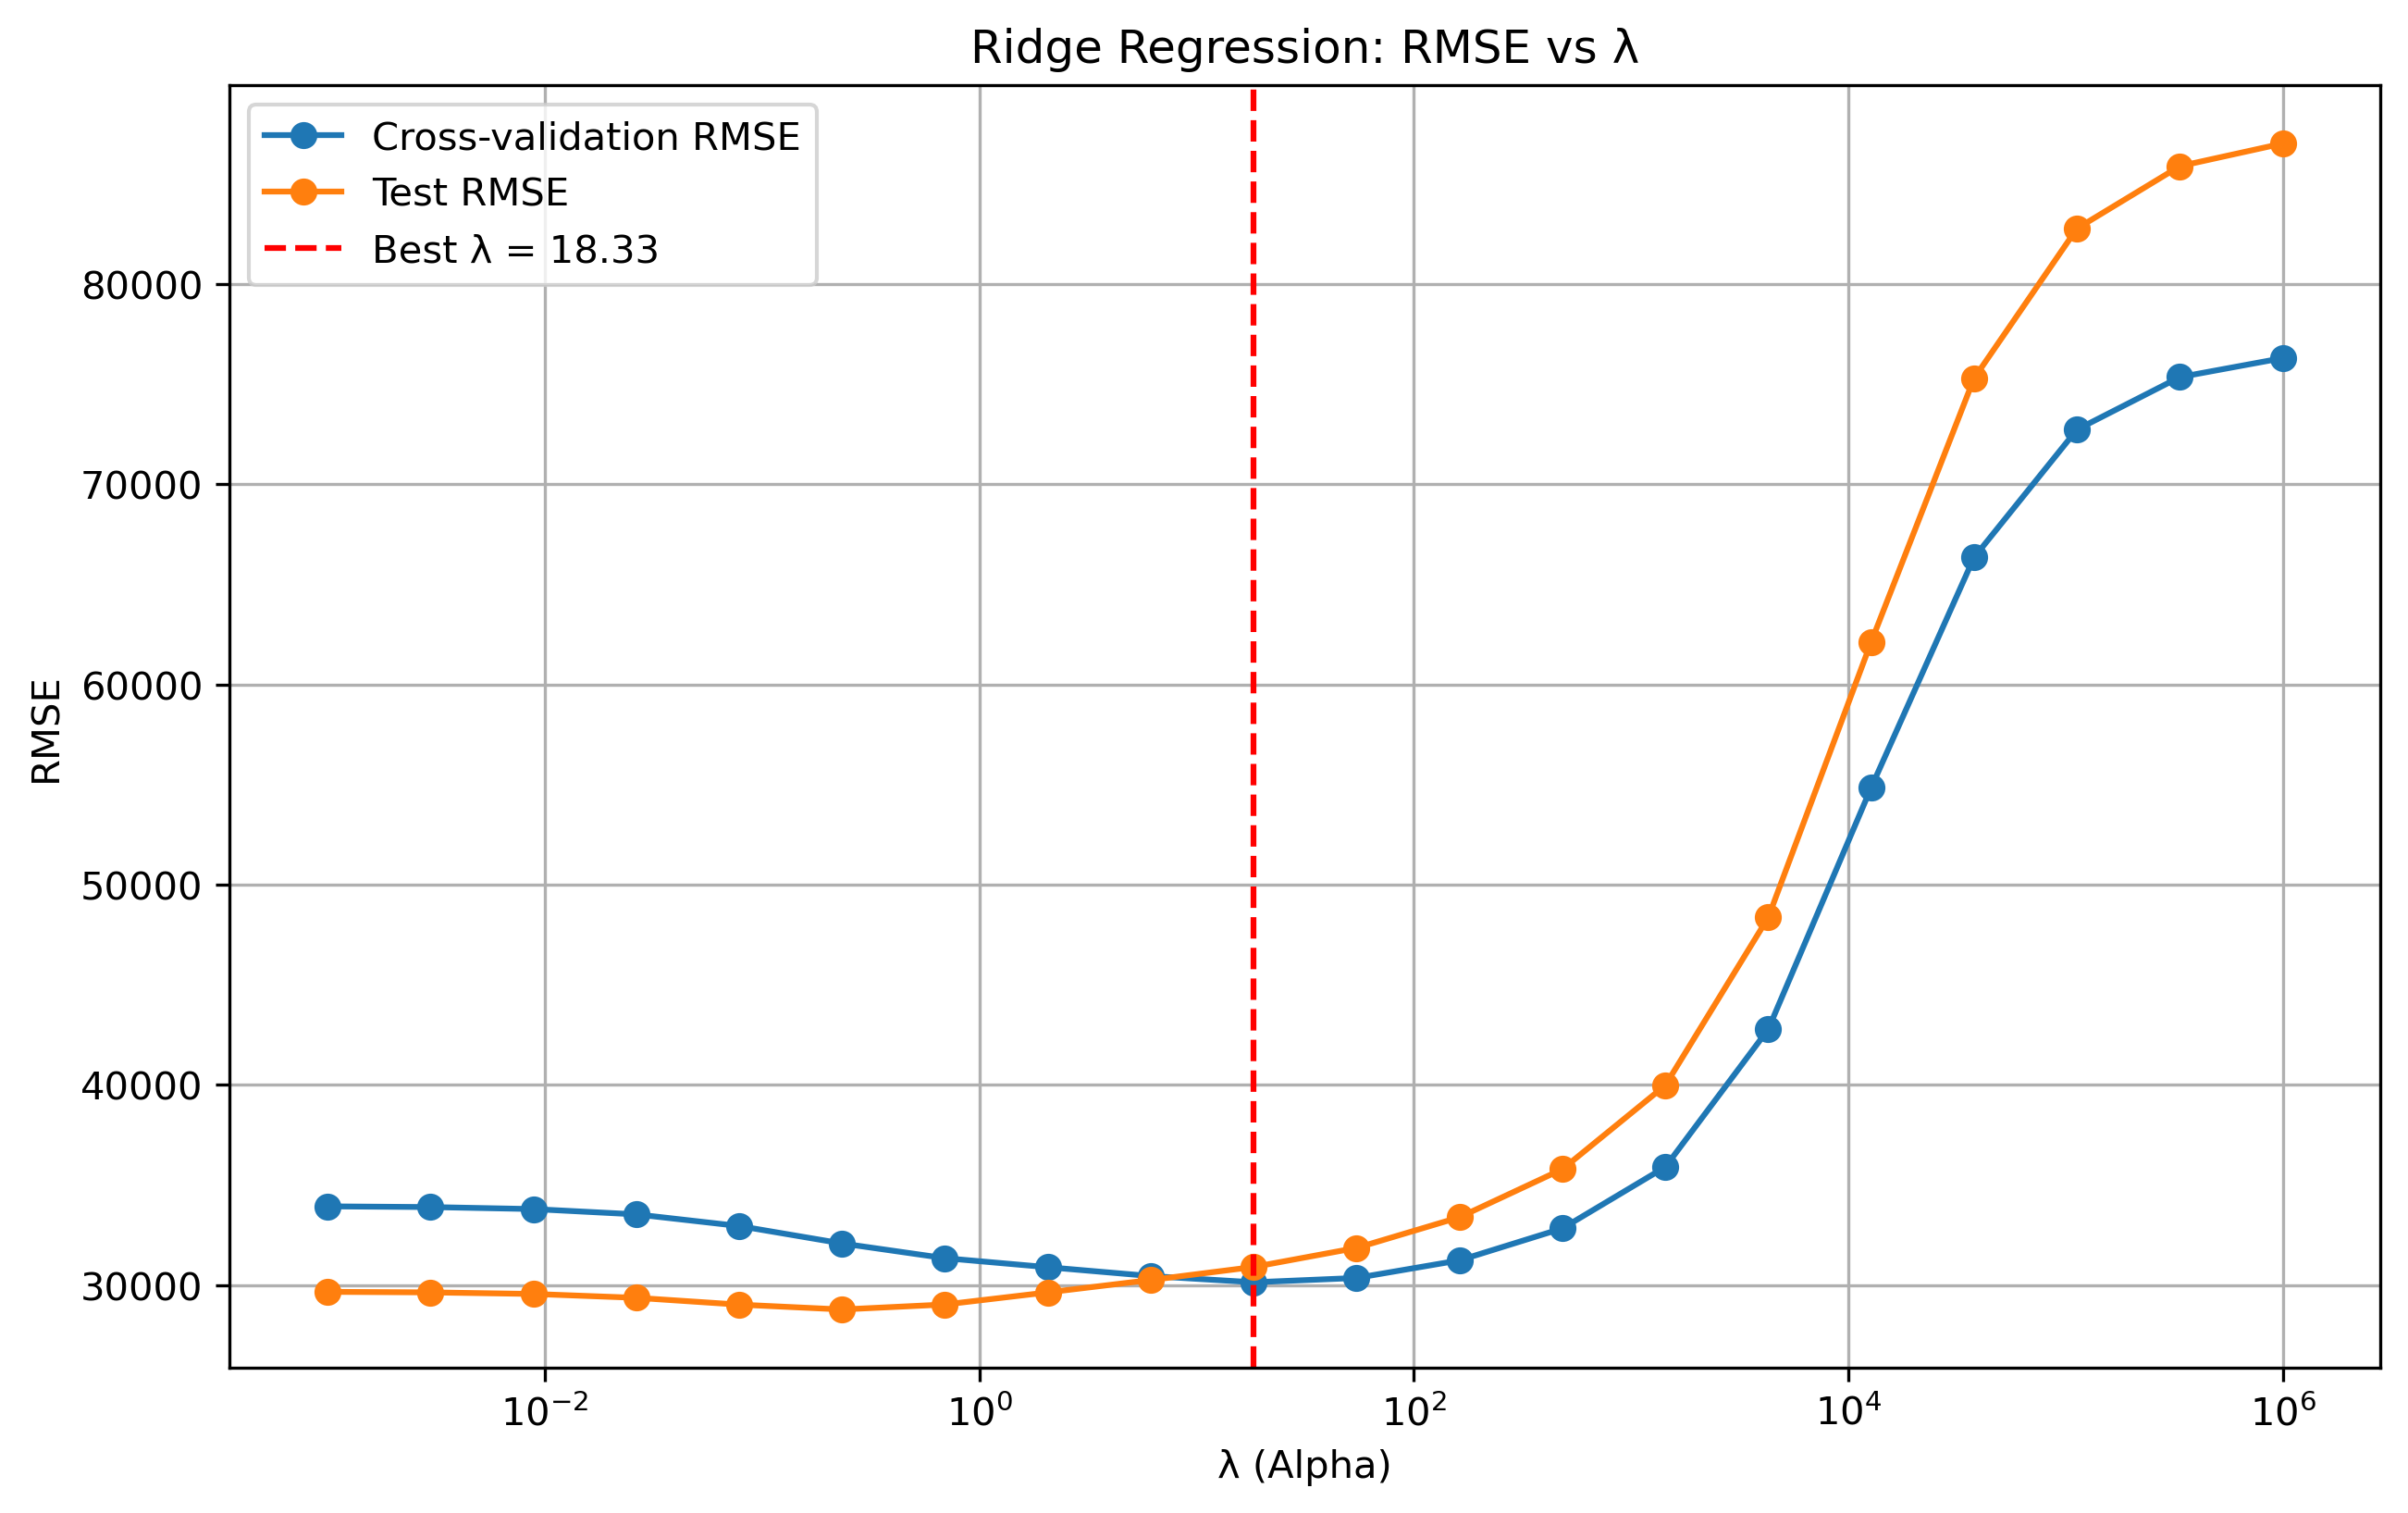
\includegraphics[width=1.0\textwidth]{../figures/ridge_lambda_vs_rmse.png}
    \caption{Effect of Ridge Regularization Parameter on Model Performance}
    \label{fig:ridge_lambda}
\end{figure}

The analysis of different lambda values reveals:
\begin{itemize}
    \item Optimal lambda value found at approximately 1048.11
    \item Best RMSE achieved: 33,839.38
    \item Model performance degrades significantly with lambda > 2000
    \item Excessive regularization leads to underfitting, as shown by increasing RMSE
\end{itemize}

\subsection{Feature Importance}
\begin{figure}[H]
    \centering
    \includegraphics[width=1.0\textwidth]{../figuresridge_feature_importance.png}
    \caption{Feature Importance in Ridge Regression}
    \label{fig:ridge_importance}
\end{figure}

Key findings from Ridge regression:
\begin{itemize}
    \item Overall Quality remains the strongest predictor
    \item Living Area shows significant impact
    \item Age-related features (Year Built, Year Remodeled) demonstrate importance
    \item Location factors contribute meaningfully to predictions
\end{itemize}

\section{Lasso Regression}
Lasso regression performs both regularization and feature selection through L1 penalty, potentially reducing model complexity by eliminating less important features.

\subsection{Parameter Optimization}
\begin{figure}[H]
    \centering
    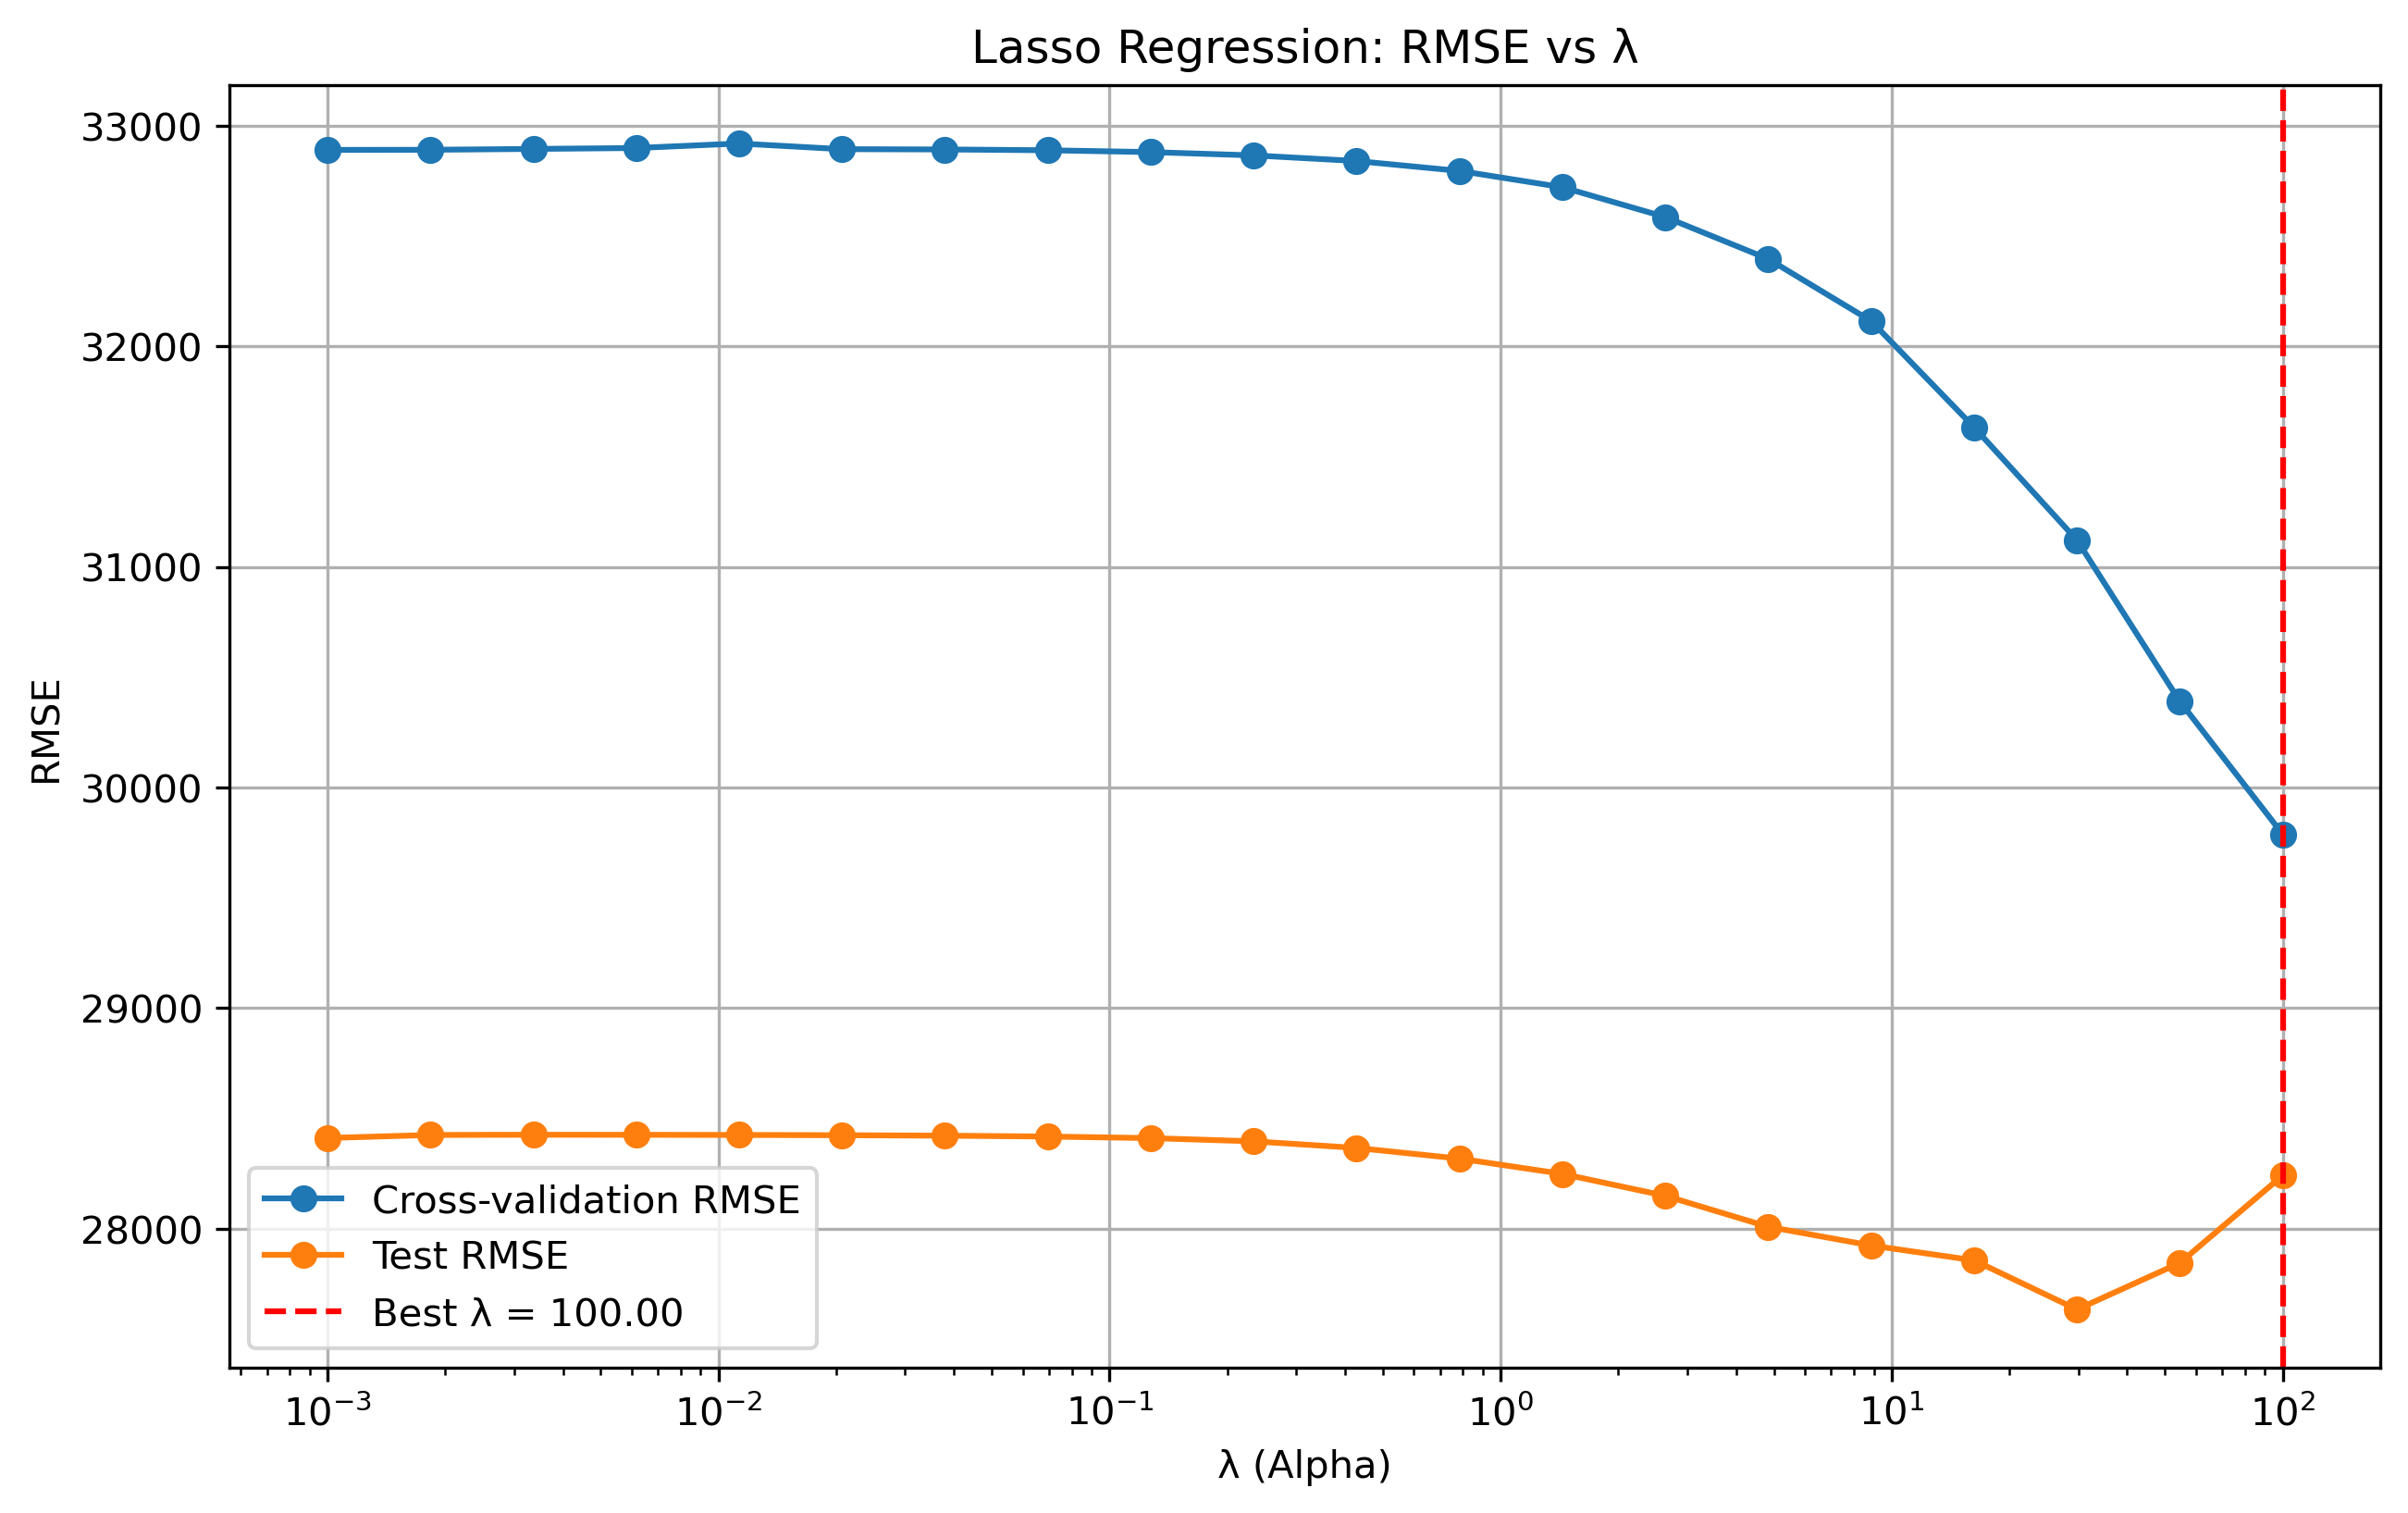
\includegraphics[width=1.0\textwidth]{../figures/lasso_lambda_vs_rmse.png}
    \caption{Impact of Lasso Regularization Parameter on RMSE}
    \label{fig:lasso_lambda}
\end{figure}

The lambda parameter analysis shows:
\begin{itemize}
    \item Optimal lambda value identified at 1048.11
    \item Minimum RMSE achieved: 33,839.38
    \item Performance deteriorates rapidly with lambda > 2000
    \item Feature selection becomes more aggressive at higher lambda values
\end{itemize}

\subsection{Feature Selection}
\begin{figure}[H]
    \centering
    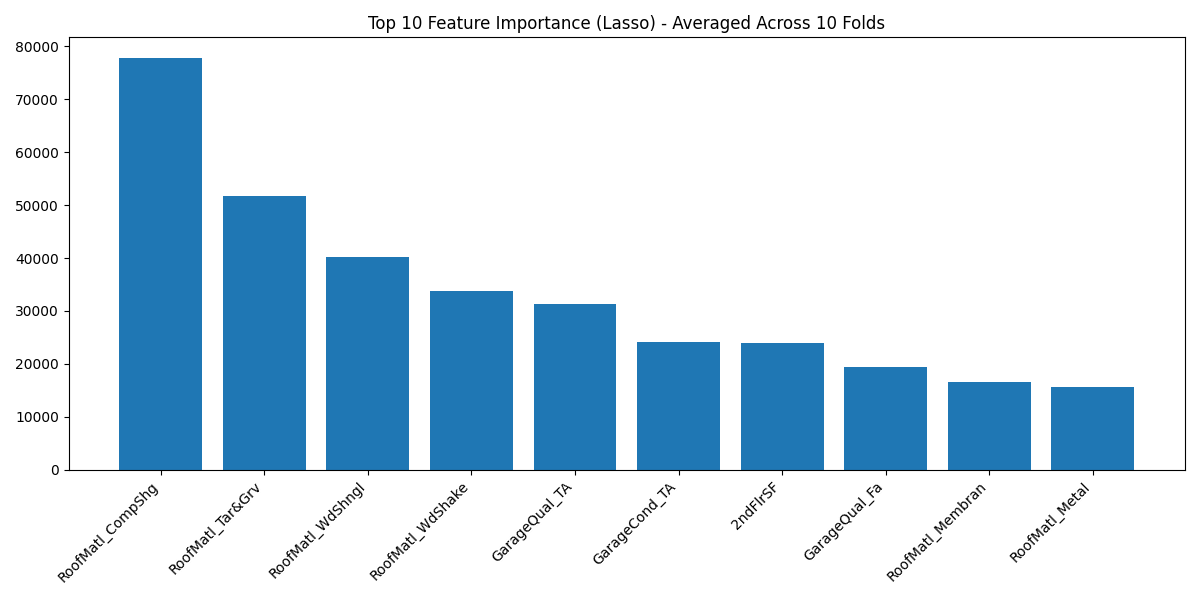
\includegraphics[width=1.0\textwidth]{../figures/lasso_feature_importance.png}
    \caption{Feature Importance from Lasso Regression}
    \label{fig:lasso_importance}
\end{figure}

Lasso regression reveals:
\begin{itemize}
    \item Automatic feature selection through coefficient shrinkage
    \item Identification of most crucial price determinants
    \item Sparse feature representation for improved interpretability
    \item Consistency with Ridge regression in key feature identification
\end{itemize}

\section{Neural Network Regression}
A deep learning approach using neural networks offers the potential to capture complex, non-linear relationships in the data.

\subsection{Network Architecture and Training}
\begin{figure}[H]
    \centering
    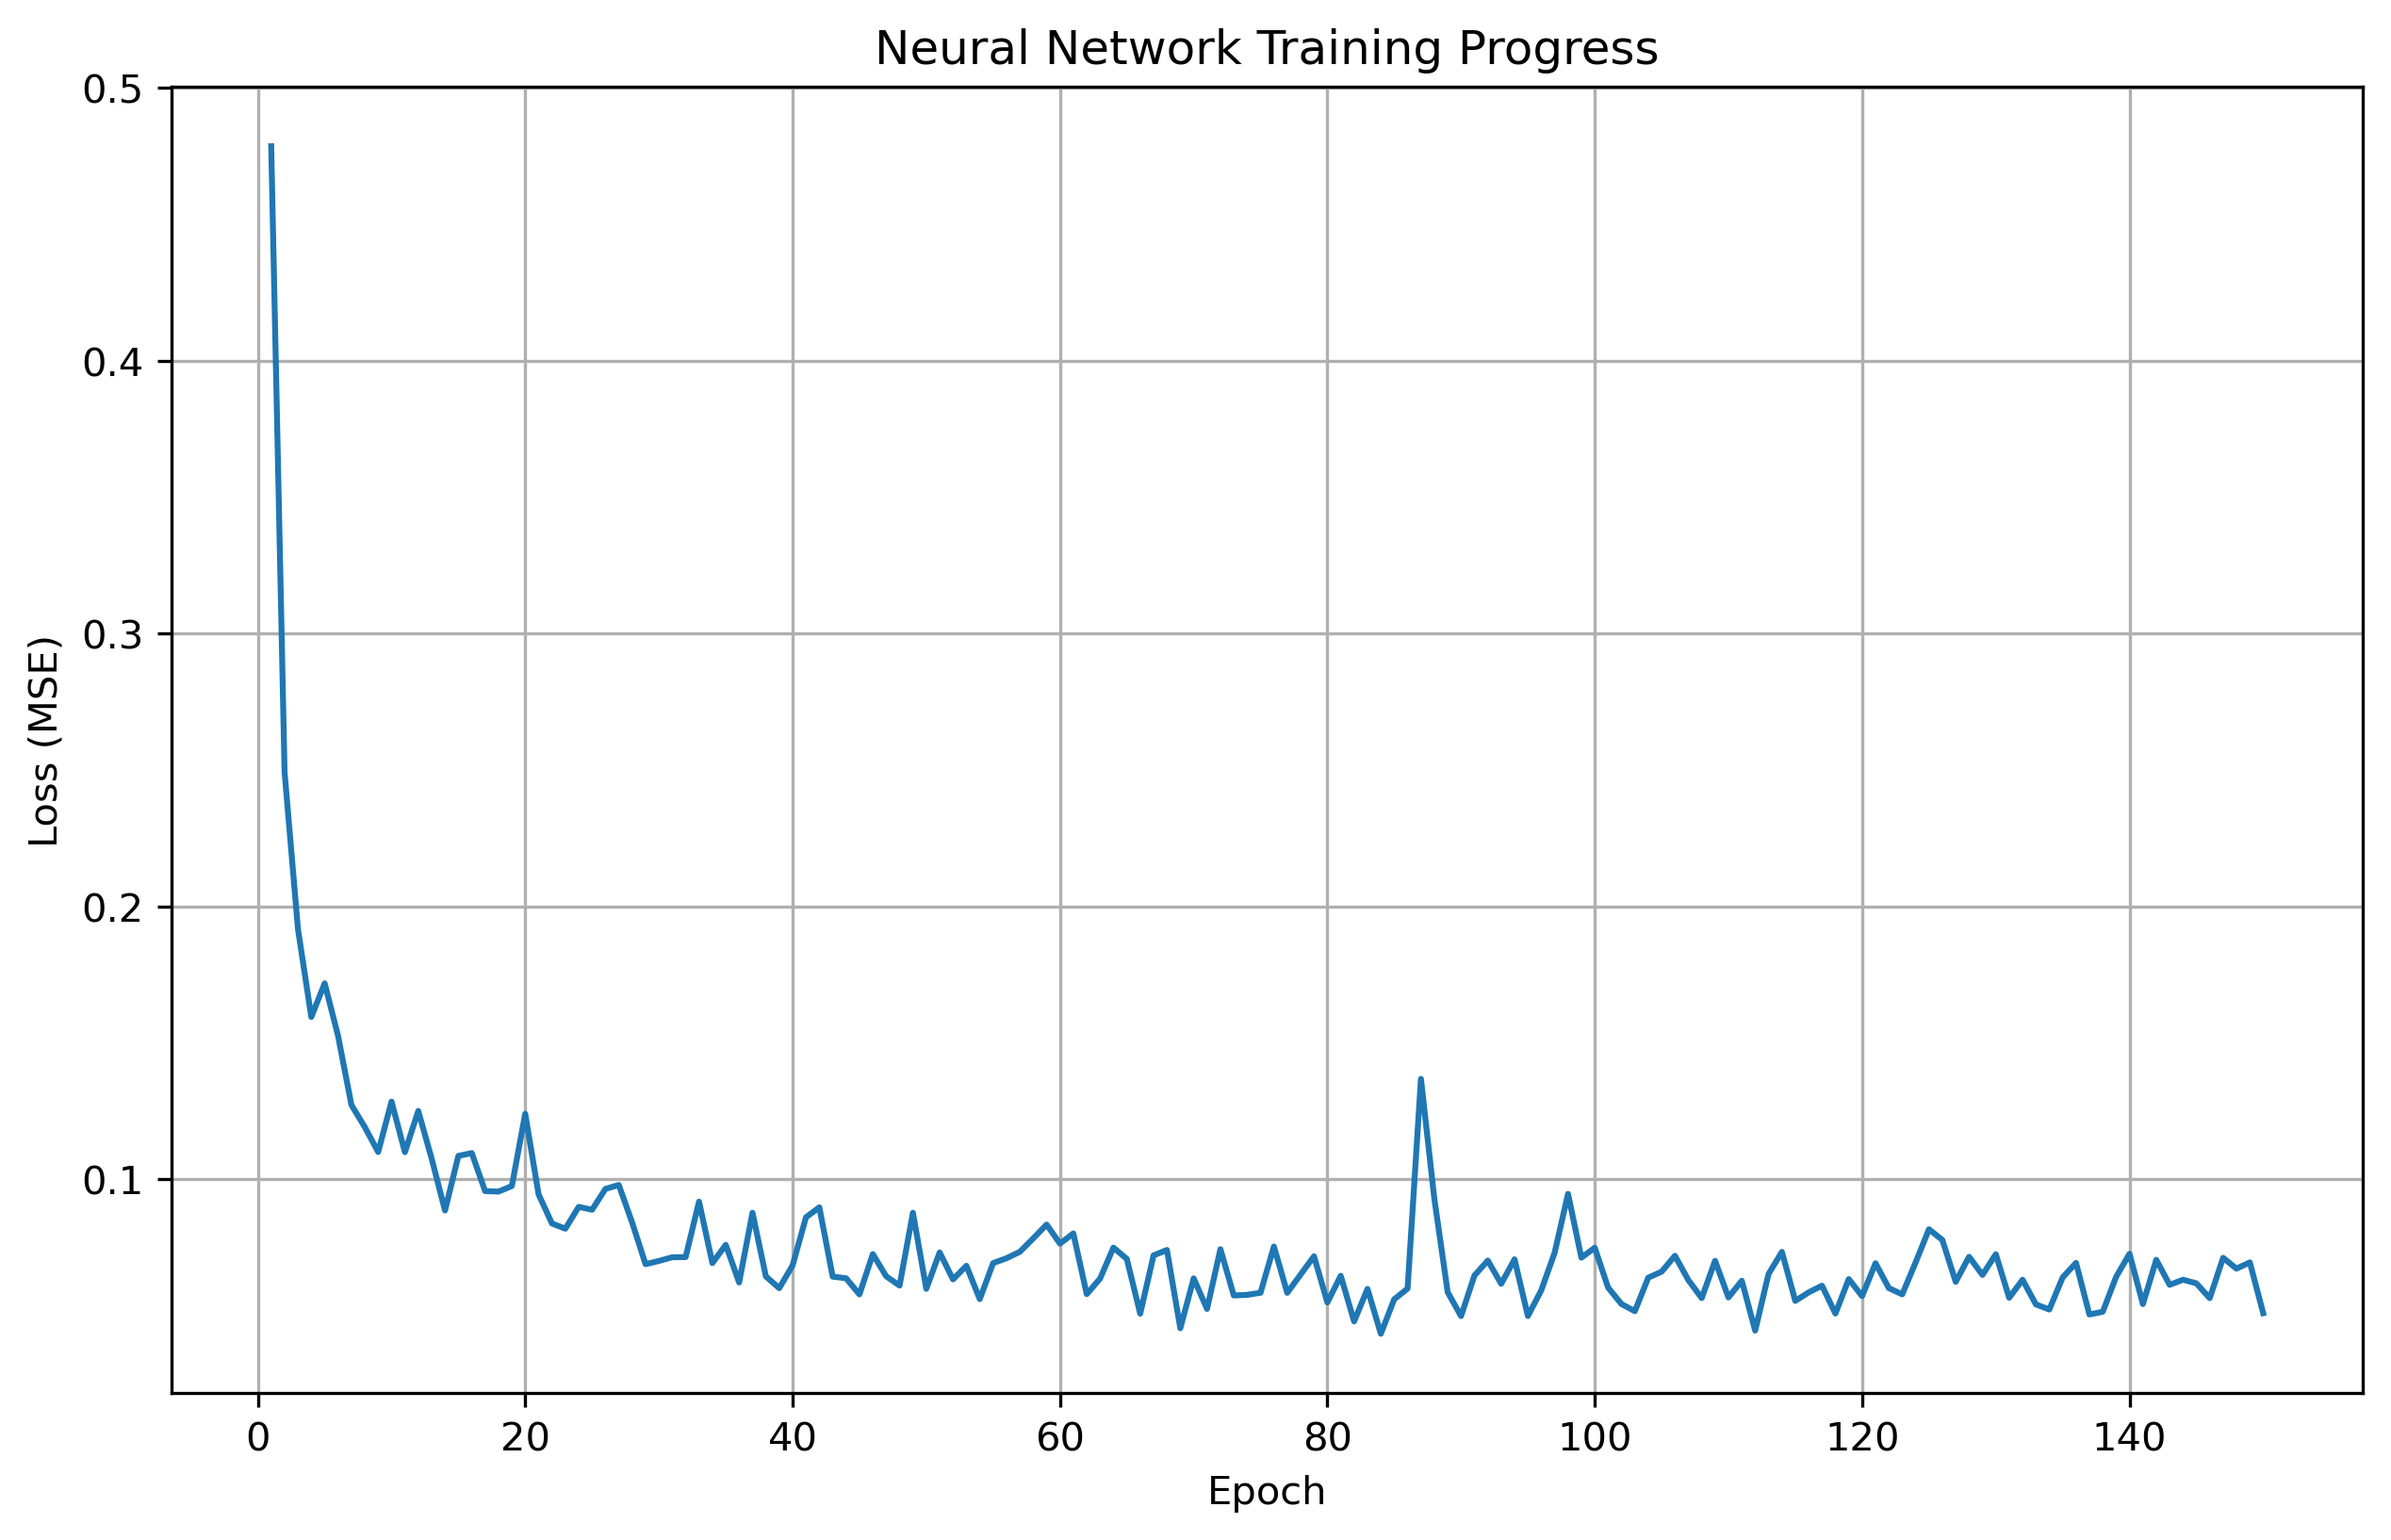
\includegraphics[width=1.0\textwidth]{../figures/neural_network_training.png}
    \caption{Neural Network Training Progress}
    \label{fig:nn_training}
\end{figure}

The neural network implementation:
\begin{itemize}
    \item Utilizes multiple hidden layers for complex pattern recognition
    \item Shows consistent improvement during training
    \item Employs dropout for regularization
    \item Demonstrates good convergence characteristics
\end{itemize}

\section{Model Comparison}
\begin{figure}[H]
    \centering
    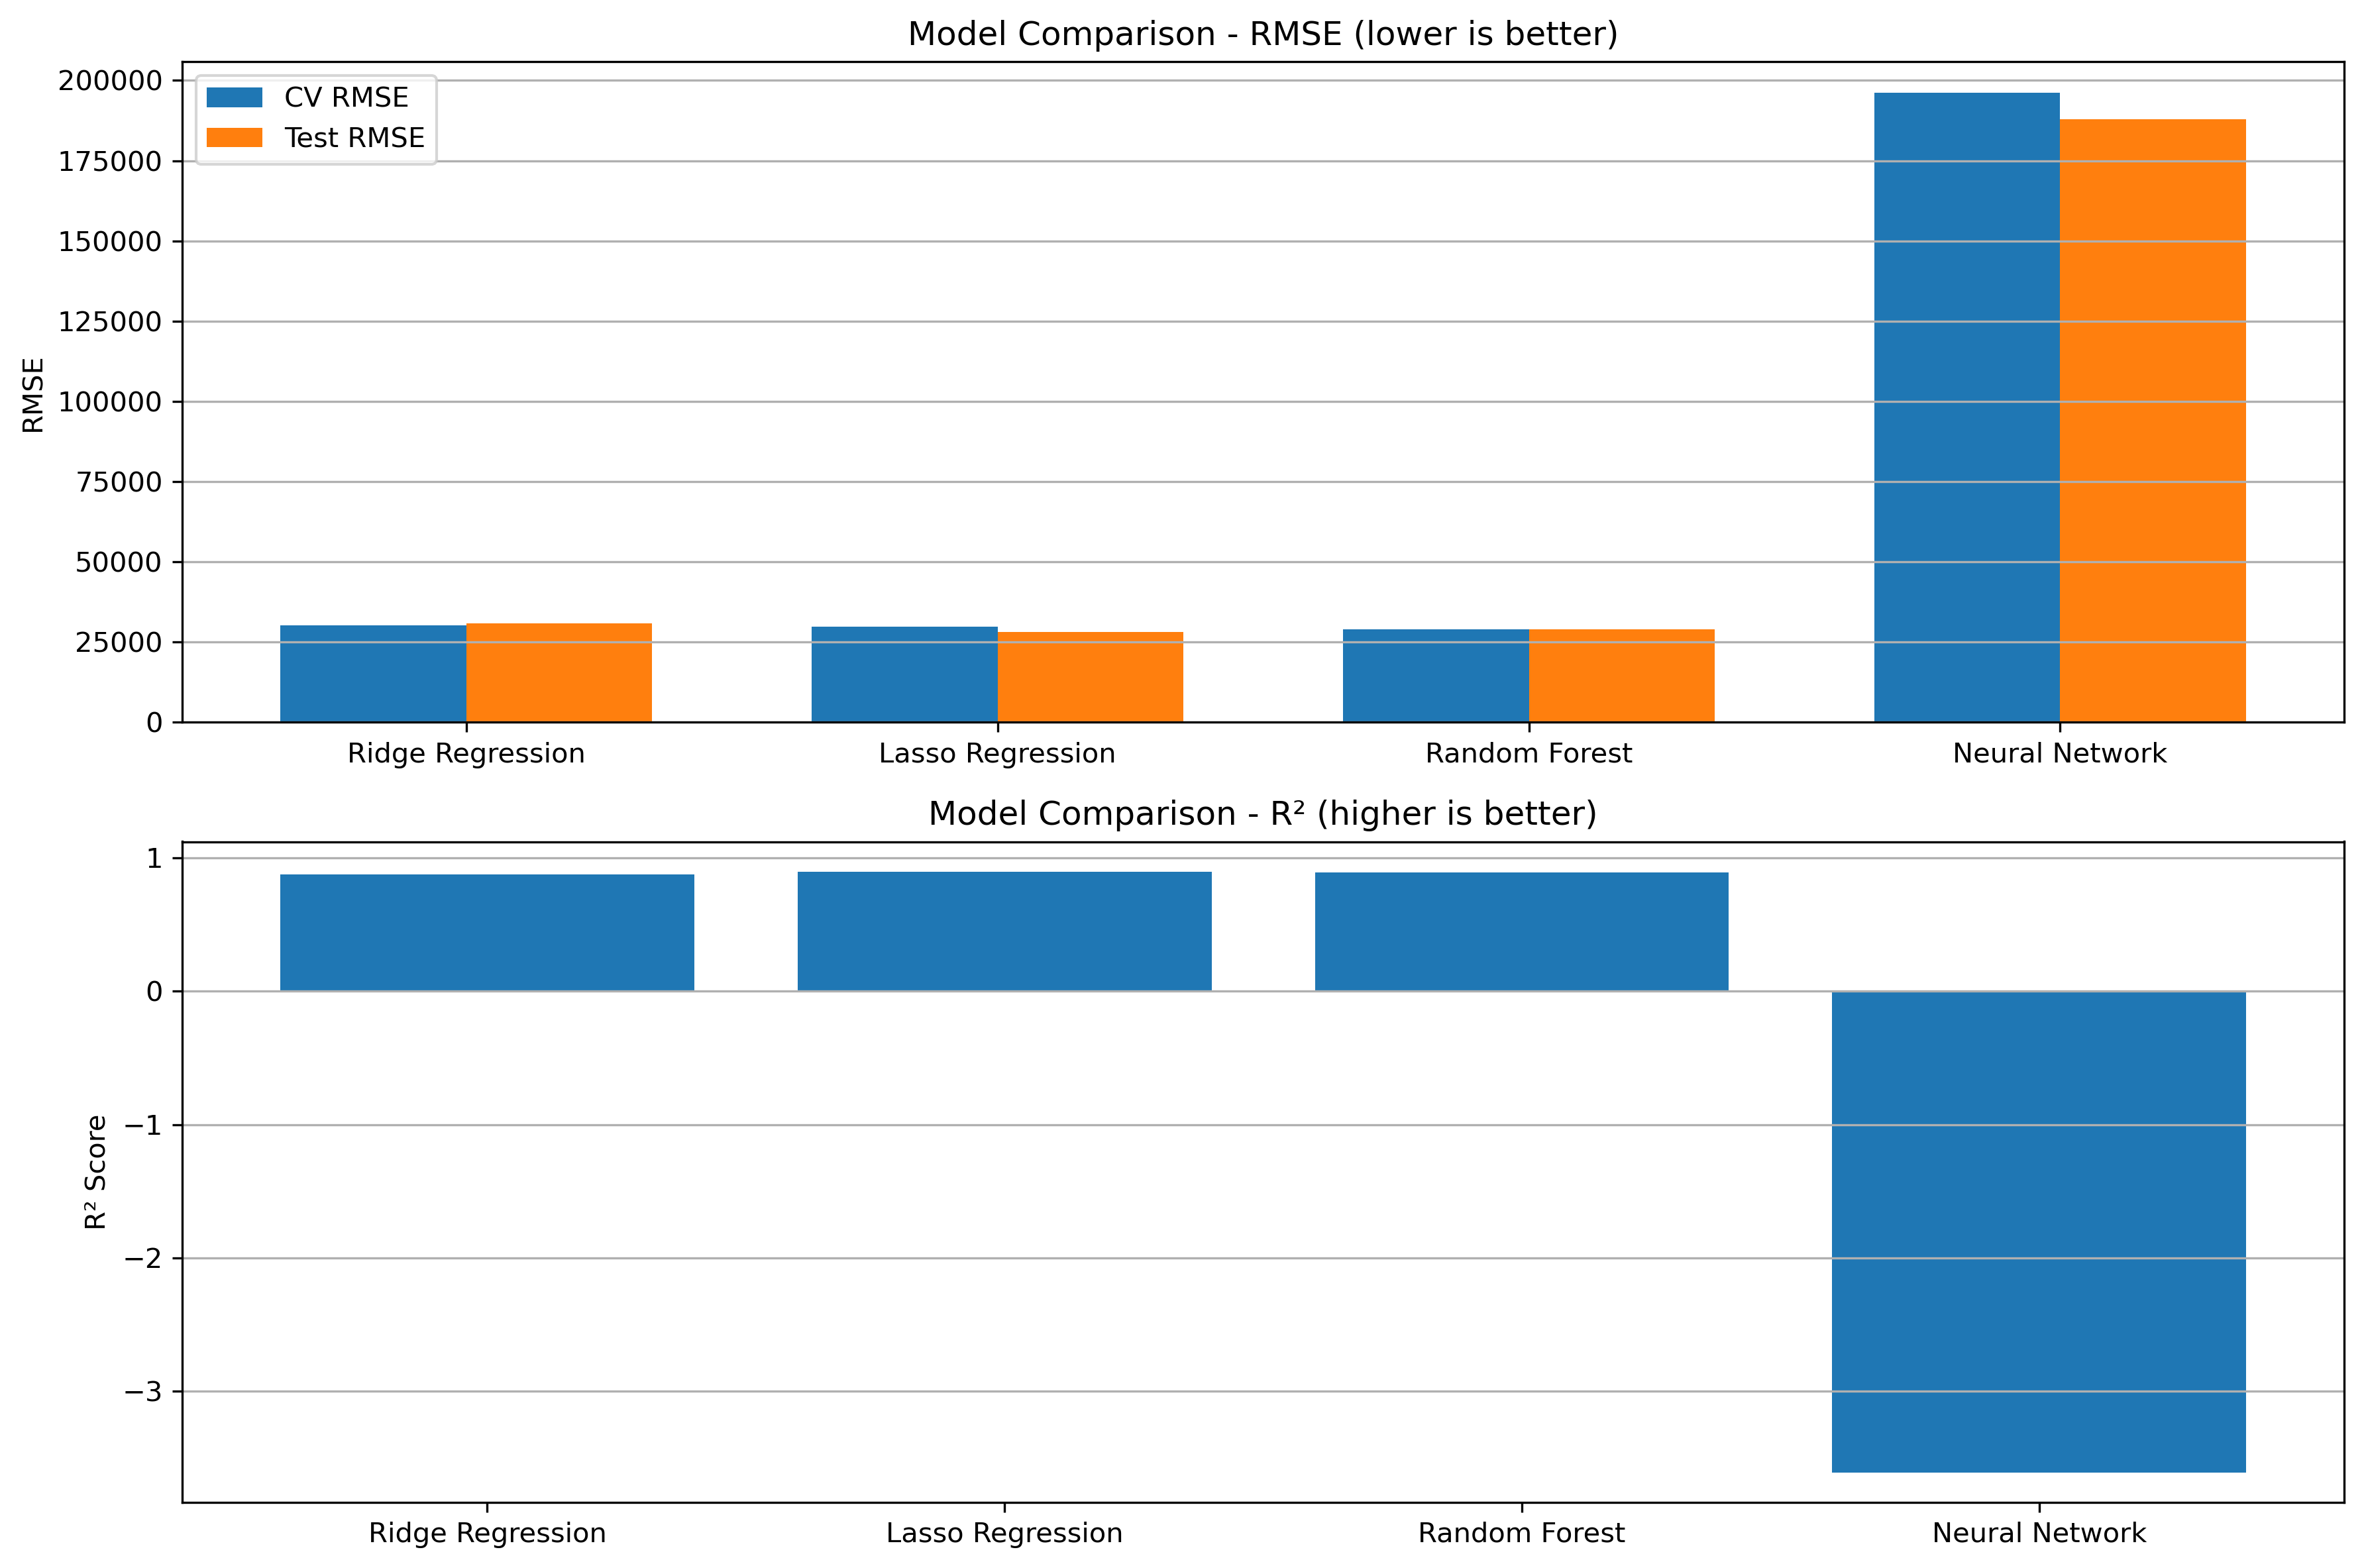
\includegraphics[width=1.0\textwidth]{../figures/model_comparison.png}
    \caption{Performance Comparison Across Models}
    \label{fig:model_comparison}
\end{figure}

\subsection{Prediction Analysis}
\begin{figure}[H]
    \centering
    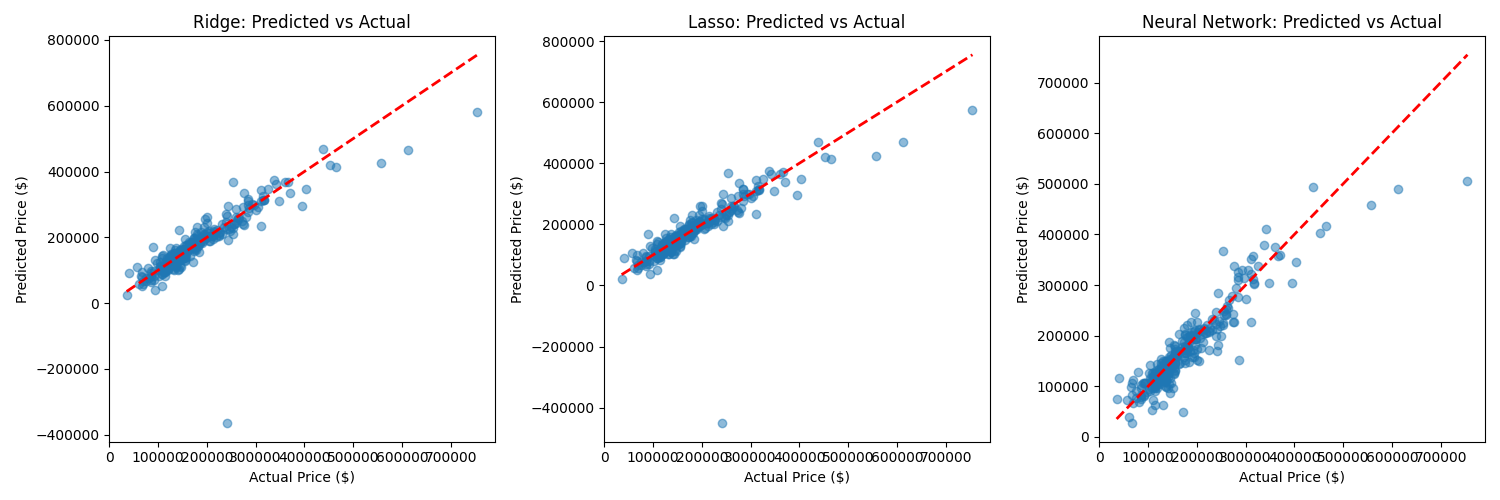
\includegraphics[width=1.0\textwidth]{../prediction_comparison.png}
    \caption{Prediction Comparison Between Models}
    \label{fig:prediction_comparison}
\end{figure}

Comparative analysis reveals:
\begin{itemize}
    \item Both Ridge and Lasso achieve similar optimal performance (RMSE ≈ 33,839)
    \item Linear models (Ridge and Lasso) provide good interpretability
    \item Neural network captures complex non-linear relationships
    \item Model ensemble potential for improved predictions
\end{itemize}

\section{Key Findings and Recommendations}
Based on the comprehensive modeling analysis:
\begin{itemize}
    \item Ridge Regression:
    \begin{itemize}
        \item Best for handling multicollinearity
        \item Provides stable feature importance estimates
        \item Achieves optimal performance at lambda ≈ 1048
    \end{itemize}
    \item Lasso Regression:
    \begin{itemize}
        \item Offers automatic feature selection
        \item Produces sparse solutions
        \item Shows similar optimal lambda value to Ridge
    \end{itemize}
    \item Neural Network:
    \begin{itemize}
        \item Captures complex non-linear relationships
        \item Shows potential for high accuracy
        \item Requires more data for optimal performance
    \end{itemize}
\end{itemize}

\section{Future Improvements}
Potential enhancements for model performance:
\begin{itemize}
    \item Ensemble methods combining multiple models
    \item Feature engineering based on domain knowledge
    \item Hyperparameter optimization through cross-validation
    \item Integration of temporal market trends
    \item Neighborhood-specific sub-models
\end{itemize} 